\documentclass[12pt,letterpaper]{article}
\usepackage{lmodern}
\usepackage[left=1.10in,right=1.10in,top=.85in,bottom=.90in]{geometry}
\usepackage[utf8]{inputenc}
\usepackage{amsmath,amssymb,amsthm,mathtools,booktabs,array,tabularx}
\usepackage{microtype}
\usepackage{tikz,graphicx,caption,xcolor,float}
\usetikzlibrary{arrows.meta,positioning,calc,decorations.pathreplacing,backgrounds}
\usepackage[numbers,sort&compress]{natbib}
\usepackage{xurl}
\usepackage[colorlinks=true,linkcolor=blue!65!black,citecolor=blue!65!black,urlcolor=blue!65!black]{hyperref}

\definecolor{ink}{HTML}{172534}
\definecolor{azure}{HTML}{245C91}
\definecolor{jade}{HTML}{087F77}
\definecolor{grayline}{HTML}{D5DEE8}
\definecolor{papergray}{HTML}{F4F7FA}
\hypersetup{pdftitle={Physical Resource Complexity of Hysteretic State Machines},pdfauthor={Rudra Tiwari},pdfsubject={Exact memory bounds and interaction-order tradeoffs for pulse-driven hysteretic finite-state machines}}
\captionsetup{font=small,labelfont=bf,justification=justified,skip=5pt}
\setlength{\parindent}{1.5em}
\setlength{\parskip}{0pt}
\setlength{\emergencystretch}{2em}
\setlength{\abovedisplayskip}{9pt plus 2pt minus 3pt}
\setlength{\belowdisplayskip}{9pt plus 2pt minus 3pt}
\setcounter{tocdepth}{2}
\newtheorem{theorem}{Theorem}[section]
\newtheorem{lemma}[theorem]{Lemma}
\newtheorem{proposition}[theorem]{Proposition}
\newtheorem{corollary}[theorem]{Corollary}
\theoremstyle{definition}\newtheorem{definition}[theorem]{Definition}
\theoremstyle{remark}\newtheorem{remark}[theorem]{Remark}
\newcommand{\wt}{\operatorname{wt}}
\newcommand{\Nmin}{N_{\min}}
\newcommand{\Kmin}{K_{\min}}
\newcommand{\ceil}[1]{\left\lceil #1\right\rceil}
\newcommand{\floor}[1]{\left\lfloor #1\right\rfloor}
\newcommand{\supp}{\operatorname{supp}}
\newcommand{\bits}{\{0,1\}}
\newcommand{\Lrank}[2]{\mathcal L^{(#1)}_{#2}}
\begin{document}
\thispagestyle{empty}
\begin{center}
\vspace*{0.26in}
{\LARGE\bfseries Physical Resource Complexity of\\[.15em] Hysteretic State Machines\par}
\vspace{.25in}
{\large Realizability, Optimal Memory, and Interaction Tradeoffs\par}
\vspace{.26in}
{\normalsize\bfseries Rudra Tiwari\par}
\vspace{.025in}
{\normalsize\itshape University of Delhi, New Delhi, India\\Inter-University Accelerator Centre (IUAC), New Delhi, India\par}
\vspace{.10in}
{\small\href{https://orcid.org/0009-0004-8521-7627}{ORCID: 0009-0004-8521-7627}\quad|\quad\href{https://rtx09x.github.io/}{Website}\quad|\quad\href{https://github.com/Rtx09x}{GitHub}\quad|\quad\href{https://github.com/Rtx09x/Open-Research/tree/main/applied-physics/hysteretic-state-machines}{Open-Research}\par}
\vspace{.16in}
{\normalsize November 2026\par}
\end{center}
\vspace{.19in}
\begin{abstract}
The number of binary states that a physical device can store does not determine which state transitions it can execute. We study the resources needed to realize a specified finite-state computation with interacting hysterons. One input is a repeated quasistatic scalar excursion; at most one element switches on during the rising half and one switches off during the falling half. This budget forces a constrained geometry on state transitions. We characterize unary transition maps realizable with unrestricted switch count, prove sharp memory bounds for cyclic, resetting, and merging behaviors, and obtain exact tradeoffs among switch count, polynomial interaction order, and directed interaction terms for one-pulse reset. A seven-state task separates pairwise from three-body interactions at three switches; a ten-state counter has exact minima of six and five switches in the respective models. We give near-capacity counter constructions for every period at least three and a finite synthesis procedure with checkable rational witnesses and infeasibility certificates. The analysis identifies the transition structure, rather than state count alone, as an independent determinant of memory cost. All results concern the stated switching-threshold model; terms and incidences are abstract resource counts, not manufacturing costs.
\end{abstract}
\vspace{.12in}
\noindent\textbf{Keywords:} hysteresis, finite-state machines, physical memory, switching constraints, interaction order, resource bounds, exact synthesis.
\clearpage
\tableofcontents
\clearpage

\section{Introduction}
\noindent\textbf{Central question.} A finite-state machine is ordinarily specified by its states and transitions. Its physical realization raises a second problem: how should those states be embedded into binary components, and what constraints does the device impose on transitions? A collection of $n$ binary switches has $2^n$ configurations, but that number alone says nothing about whether one repeated physical input can move between selected configurations in the desired order.

Hysterons, elements with different thresholds for switching on and off, provide a minimal model of physical memory \citep{preisach1935,liu2024}. Their interactions alter those thresholds as the surrounding configuration changes. General transition-graph synthesis and feasibility inequalities have already been developed \citep{teunisse2025}; dynamical self-loops and energy-injection effects have also been characterized \citep{baconnier2025}; catastrophe-theoretic designs provide a complementary route to transition pathways \citep{muhaxheri2025}, and mechanical networks with designed couplings provide experimental motivation \citep{shohat2025,paulsen2026,ali2026}. Our question is more restricted: \emph{what can be proved about the number of memory elements and the interaction structure needed for a prescribed machine when each pulse is allowed only a small number of individual switches?}

The limitation is intentionally strong. A logical input is always the same scalar excursion $L\nearrow H\searrow L$. The increasing branch permits at most one $0\to1$ flip; the decreasing branch permits at most one $1\to0$ flip. Avalanche size is counted in individual switches. We neither vary the pulse in response to the current state nor introduce a hidden controller. This restricted setting permits sharp statements without implying universal limits on computers or arbitrary mechanical devices.

The paper follows one dependency chain. \emph{Transition geometry} identifies the only allowable movements between codes (Section~\ref{sec:geometry}). This gives \emph{realizability criteria} and \emph{capacity bounds} (Sections~\ref{sec:real} and \ref{sec:cycles}). Those bounds become exact \emph{memory laws} for specified tasks (Section~\ref{sec:tasks}). Finally, restricting the degree and support of threshold interactions produces \emph{joint resource tradeoffs} and concrete separations (Sections~\ref{sec:frontier} and \ref{sec:separation}). An exact decision procedure and replayable certificates connect the mathematical claims to computation (Section~\ref{sec:algorithm}).

This approach is related to the long-standing finite-state \emph{state-assignment} problem \citep{ahmad2000}. It differs in its objective and constraint set: rather than minimizing a logic circuit after encoding the states, it optimizes binary hysterons under a quasistatic event budget and threshold-coupling restrictions. No novelty is claimed for the general notions of state encoding, linear-feasibility testing, or Boolean-function representation.

\begin{figure}[H]
\centering
\resizebox{.98\linewidth}{!}{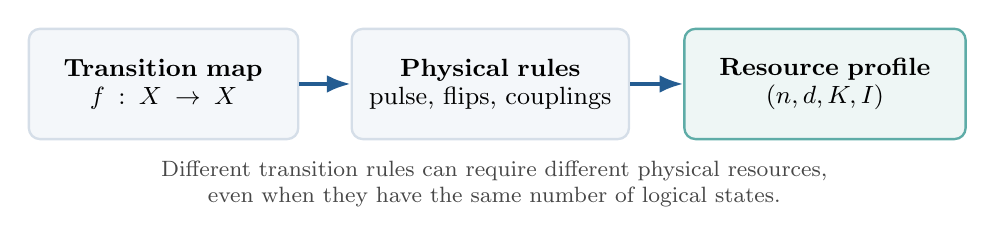
\begin{tikzpicture}[>=Latex,font=\small,x=1cm,y=1cm]
\tikzset{b/.style={draw=grayline,line width=.85pt,rounded corners=4pt,fill=papergray,minimum height=1.4cm,align=center,inner sep=6pt},a/.style={-{Latex[length=3mm]},line width=1.25pt,draw=azure}}
\node[b,text width=3.0cm] (a) at (0,0) {\textbf{Transition map}\\[-1pt]$f:X\rightarrow X$};
\node[b,text width=3.1cm] (b) at (4.15,0) {\textbf{Physical rules}\\[-1pt]pulse, flips, couplings};
\node[b,text width=3.15cm,draw=jade!65,fill=jade!7] (c) at (8.4,0) {\textbf{Resource profile}\\[-1pt]$(n,d,K,I)$};
\draw[a] (a.east)--(b.west);
\draw[a] (b.east)--(c.west);
\node[font=\footnotesize,align=center,text=black!72] at (4.2,-1.27) {Different transition rules can require different physical resources,\\even when they have the same number of logical states.};
\end{tikzpicture}
}
\caption{The research problem. A transition map specifies what must happen; hysteresis and a per-pulse switching budget constrain its encoding. The resource profile measures switch count $n$, polynomial degree $d$, term support $K$, and source incidences $I$.}
\label{fig:overview}
\end{figure}

\section{Model and resource measures}\label{sec:model}
Let $[n]=\{1,\ldots,n\}$ index $n$ binary hysterons. A physical configuration $S\subseteq[n]$ records its active elements; equivalently $s\in\bits^n$. For an element $i$ and the environment $E\subseteq[n]\setminus\{i\}$, let $U_i^+(E)$ and $U_i^-(E)$ denote its upward and downward switching fields. For a full configuration $S$, $U_i^{\pm}(S)$ abbreviates $U_i^{\pm}(S\setminus\{i\})$. We require a positive span in \emph{every} Boolean environment:
\begin{equation}\label{eq:span}
 U_i^+(E)>U_i^-(E) \qquad (i\in[n],\ E\subseteq[n]\setminus\{i\}).
\end{equation}
At an instantaneous field $h$, a configuration is strictly stable when
\begin{equation}\label{eq:stable}
 h<U_i^+(S)\ \ (i\notin S), \qquad h>U_i^-(S)\ \ (i\in S).
\end{equation}
On an increasing quasistatic ramp the off element with the lowest upward threshold triggers first; on a decreasing ramp the on element with the highest downward threshold triggers first. Switching recalculates the remaining thresholds. All operating comparisons are strict, so there is no tie-dependent transition rule.

\begin{figure}[ht]
\centering\resizebox{\linewidth}{!}{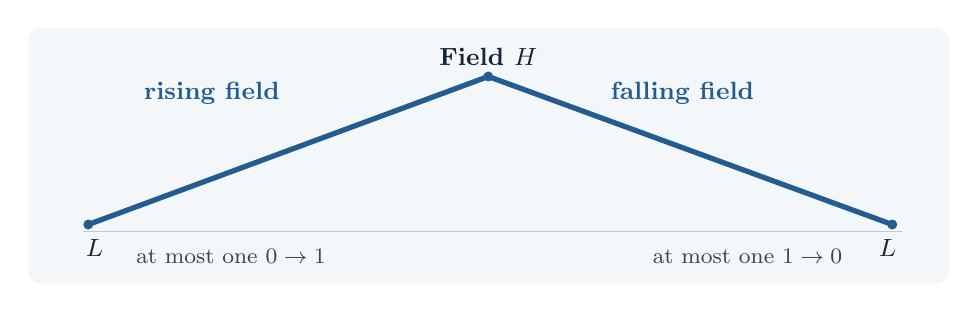
\begin{tikzpicture}[>=Latex,x=1cm,y=1cm,font=\small]
\fill[papergray,rounded corners=5pt] (0,0) rectangle (11.7,3.25);
\draw[black!22] (.70,.66)--(11.1,.66);
\draw[azure,line width=1.9pt,line cap=round,line join=round] (.77,.75)--(5.85,2.63)--(10.98,.75);
\fill[azure] (.77,.75) circle (1.8pt);
\fill[azure] (5.85,2.63) circle (1.8pt);
\fill[azure] (10.98,.75) circle (1.8pt);
\node[above,text=ink,font=\bfseries\small] at (5.85,2.65) {Field $H$};
\node[below,text=ink] at (.85,.68) {$L$};
\node[below,text=ink] at (10.92,.68) {$L$};
\node[rotate=0,anchor=center,font=\small\bfseries,text=azure] at (2.34,2.42) {rising field};
\node[anchor=east,font=\small\bfseries,text=azure] at (9.35,2.42) {falling field};
\node[font=\footnotesize,text=black!74] at (2.58,.35) {at most one $0\to1$};
\node[font=\footnotesize,text=black!74] at (9.14,.35) {at most one $1\to0$};
\end{tikzpicture}
}
\caption{One logical input consists of the increasing \emph{and} decreasing halves of the same field pulse. The allowed switching budget is one individual flip on each half, not one flip for the entire pulse.}
\label{fig:pulse}
\end{figure}

\begin{definition}[Budgeted realization]
For a nonempty finite state set $X$ and a successor map $f:X\to X$, a realization comprises an injective encoding $C:X\hookrightarrow 2^{[n]}$ and a pulse $L\nearrow H\searrow L$ such that every code $C(x)$ is stable at $L$, and the pulse maps $C(x)$ to $C(f(x))$ with at most one individual flip on each half. A logical fixed point may execute an internal $0\to1\to0$ excursion unless an additional condition forbids it.
\end{definition}
Initialization, measurement, timing, fabrication, energy dissipation, and behavior at undesignated initial states are \emph{not} included in this realization criterion. These exclusions are relevant when interpreting physical cost.

The threshold interactions are represented by multilinear polynomials:
\begin{equation}\label{eq:poly}
 U_i^{\pm}(s)=u_i^{\pm}+\sum_{\substack{\emptyset\ne A\subseteq[n]\setminus\{i\}\\|A|\le d}}
 c_{i,A}^{\pm}\prod_{j\in A}s_j.
\end{equation}
Degree $d=0$ means independent hysterons; degree $1$ permits pairwise interactions; degree $2$ permits joint three-body effects. A degree-$d$ term involves $d$ input bits and one receiving bit. Coefficients may be directed, of either sign, nonreciprocal, and independently chosen on both branches unless an additional assumption is stated. \emph{Common shifts} mean $c^+_{i,A}=c^-_{i,A}$ for all nonempty $A$. Coefficients that increase the thresholds are called inhibitory for upward switching, but this convention does not assert a corresponding sign of a physical force.

\begin{definition}[Resource profile]
For a realized map $f$, write $n$ for switch count, $d$ for maximum monomial degree, and
\begin{equation}\label{eq:costs}
 K=\#\{(i,A):A\ne\emptyset,\ c^+_{i,A}\ne0\ \text{or}\ c^-_{i,A}\ne0\},\qquad
 I=\sum_{(i,A)\in\supp}|A|.
\end{equation}
We call $(n,d,K,I)$ a resource point. In particular, $K$ counts distinct directed nonconstant monomials and $I$ counts their total source incidences. The resource profile $\mathcal R(f)$ is the set of its realizable resource points, ordered by componentwise comparison. The lower envelope in a chosen coordinate defines the corresponding minimum $\Nmin^{(d)}(f)$ or $\Kmin(f;n,d)$.
\end{definition}

The profile is a mathematical accounting device, not a claim that one monomial equals one physical coupler. The interaction order, signed coefficients, incidence count and geometry of an eventual apparatus can have very different manufacturing costs.

\section{Geometry before interaction: a normal form}\label{sec:geometry}
A pulse's two allowed flips restrict the shape of every transition independently of the threshold formula.

\begin{lemma}[Budgeted transition normal form]\label{lem:normal}
Every nonfixed transition $A\to T$ adds exactly one element. It either deletes exactly one element afterwards or deletes none. Thus
\begin{equation}\label{eq:shape}
 |T\setminus A|=1,\qquad |A\setminus T|\le1.
\end{equation}
An addition-only target is fixed by the next pulse. Along any nontrivial periodic orbit the two flips are both present, so the code weight $\wt(A)=|A|$ is constant.
\end{lemma}
\begin{proof}
Initially stable on bits cannot become unstable simply by increasing the field while the state is unchanged; the first upward event, if any, is therefore an addition. If no addition occurs the downward return changes nothing. If an addition occurs but no deletion follows, its peak is stable over the driven interval and is fixed on the next pulse. Otherwise there is exactly one addition and one deletion, as required by the budget. Baseline weight is nondecreasing. It must therefore be constant around any nontrivial cycle.
\end{proof}

\begin{figure}[ht]
\centering\resizebox{\linewidth}{!}{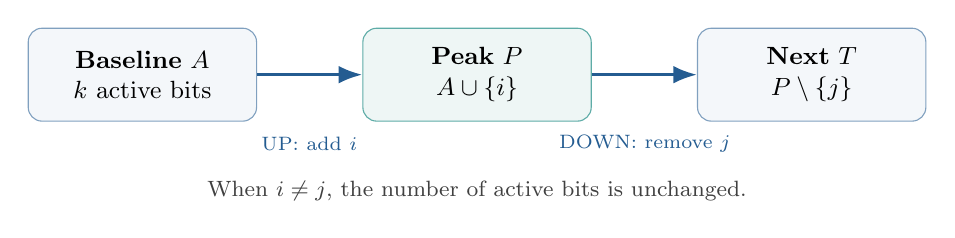
\begin{tikzpicture}[>=Latex,x=1cm,y=1cm,font=\small]
\tikzset{state/.style={draw=azure!58,fill=azure!5,rounded corners=5pt,minimum height=1.18cm,minimum width=2.9cm,align=center,inner sep=4pt},arr/.style={-{Latex[length=3mm]},line width=1.1pt,draw=azure}}
\node[state] (a) at (0,0) {\textbf{Baseline} $A$\\$k$ active bits};
\node[state,draw=jade!65,fill=jade!7] (p) at (4.25,0) {\textbf{Peak} $P$\\$A\cup\{i\}$};
\node[state] (t) at (8.5,0) {\textbf{Next} $T$\\$P\setminus\{j\}$};
\draw[arr] (a.east)--(p.west);
\draw[arr] (p.east)--(t.west);
\node[font=\scriptsize,text=azure] at (2.12,-.88) {UP: add $i$};
\node[font=\scriptsize,text=azure] at (6.38,-.88) {DOWN: remove $j$};
\node[font=\footnotesize,text=black!75] at (4.25,-1.48) {When $i\ne j$, the number of active bits is unchanged.};
\end{tikzpicture}
}
\caption{A transition with an addition passes through a peak $P$ containing one added bit. When $i\ne j$ the two logical configurations have the same number of active elements; when $i=j$, the state is fixed after the pulse and may have undergone a returning excursion.}
\label{fig:geometry}
\end{figure}

An exchange transition $A\to T$ has an intermediate peak $P=A\cup T$ of weight $|A|+1$. The same peak cannot descend to two different destinations, because dynamics are deterministic. Furthermore, the peak cannot itself be a baseline-stable logical code if its intended descent occurs above $L$.

\begin{theorem}[Encoding geometry criterion]\label{thm:criterion}
An injective code $C$ permits a realization with unrestricted threshold tables if and only if every nonfixed edge $A=C(x)\to T=C(f(x))$ satisfies all of the following:
\begin{enumerate}
\item $|T\setminus A|=1$ and $|A\setminus T|\le1$;
\item an addition-only transition reaches a fixed logical state;
\item an exchange peak $P=A\cup T$ is not itself a code;
\item all nonfixed transitions using the same peak have the same target.
\end{enumerate}
Positive spans and globally separated upward/downward threshold bands may be imposed in the realizing tables.
\end{theorem}
\begin{proof}
Necessity follows from Lemma~\ref{lem:normal}, stability of the peak, and deterministic descent. For sufficiency, label each required upward code-to-peak edge and each required downward peak-to-code edge; the four conditions make the labeling consistent. Choose $L=0$, $H=3$, and distinct $0<\eta_i<1/8$. For each other-bit environment $E$, assign
\begin{align}\label{eq:tableconstruction}
U_i^+(E)&=\begin{cases}2+\eta_i,&E\to E+i\text{ labeled up},\\4+\eta_i,&\text{otherwise},\end{cases}\\
U_i^-(E)&=\begin{cases}1+\eta_i,&E+i\to E\text{ labeled down},\\-2+\eta_i,&\text{otherwise}.\end{cases}\nonumber
\end{align}
All codes are stable at zero. The unique selected upward event occurs below $H$, and the unique selected downward event, when prescribed, occurs on the return. No other event is eligible before the endpoint. An addition-only peak is a fixed code; a required descending peak is not a code. All global spans are positive and all downward thresholds lie below all upward thresholds. Exact event-by-event inequalities follow directly from the four chosen levels.
\end{proof}

This criterion is about \emph{unrestricted} switching tables. A geometrically admissible code may still be impossible with pairwise or other degree-limited interactions. Distinguishing these two levels is essential to the rest of the paper.

\section{Which finite one-input machines exist?}\label{sec:real}
\begin{theorem}[Unary realizability]\label{thm:unary}
A finite one-input transition map $f:X\to X$ is realizable on some number of budgeted hysterons if and only if it contains no directed two-cycle between distinct states. Every admissible map on $m=|X|$ states has a realization on $m$ switches with nonnegative, common pairwise shifts and a uniform hysteresis span.
\end{theorem}
\begin{proof}
A two-cycle would consist of two same-weight exchanging codes. Both would pass through their unique common one-bit larger peak, whose descent cannot choose two different targets. This proves necessity.

For sufficiency, use the one-hot codes $C(i)=\{i\}$. For a nonfixed edge $i\to j$, assign $J_{ji}=1$ and $J_{ij}=5$; give other off-diagonal entries the value $3$. These prescriptions conflict only if $i\leftrightarrow j$ is a two-cycle. Let $B=1+\max_i\sum_{j\ne i}J_{ij}$, and use
\begin{equation}\label{eq:onehot}
 U_i^+=B+\eta_i+\sum_jJ_{ij}s_j,\qquad U_i^-=-4+\eta_i+\sum_jJ_{ij}s_j,
\end{equation}
with $L=0$, $H=B+2$, and $0<\eta_i<1/8$ distinct. At $\{i\}$ the chosen successor $j$ is the unique first addition. At $\{i,j\}$ the original bit $i$ has downward threshold $1+\eta_i$, while $j$ remains on; the pulse ends at $\{j\}$. A fixed state has no eligible addition. Positive widths, inhibitory couplings and global band separation prevent avalanches. These assertions are elementary threshold comparisons, also checked by the supplied code.
\end{proof}

The theorem settles \emph{existence with an unrestricted switch budget}. It does not say that $m$ is optimal or that a particular physical coupling geometry can implement the design. With enough memory bits, pairwise terms already realize every permitted unary map; higher-order interactions matter for \emph{compression}, not for expanding this unary existence class.

\section{Cycles, capacity and long counters}\label{sec:cycles}
For a period-$q$ cycle, the $q$ low states have common weight $k$, and the $q$ peaks have weight $k+1$. Since both sets are distinct,
\begin{equation}\label{eq:capacity}
 q\le \min\!\left\{\binom{n}{k},\binom{n}{k+1}\right\}
 \le Q(n):=\binom{n}{\floor{(n-1)/2}}.
\end{equation}
This bound is stronger than the ordinary information bound $q\le2^n$. It also excludes a two-cycle entirely, since two exchanging states have only one common peak.

A polynomial construction turns an admissible alternating cycle in Boolean layers $k,k+1$ into thresholds. Label each upward incidence with $0$, each chosen downward incidence with $4$, and the remaining incidences with $2$. For each recipient $i$, sum the corresponding degree-$k$ monomials. An appropriate uniform base threshold and hysteresis width make the desired edges the strict winners. This is an explicit synthesis rule, not merely a graph-existence argument. The full threshold form and event inequalities are recorded in Appendix~\ref{app:compiler}.

The needed combinatorial cycles are provided by established results on adjacent levels of the Boolean lattice \citep{mutzesu2017,mutze2016}. Combining that mathematics with the switching construction yields:
\begin{theorem}[Sharp rich-interaction cycle capacity]\label{thm:capacity}
For $n\ge3$, the maximum number of states in a nontrivial counter permitted by the switching budget is
\begin{equation}\label{eq:sharp}
 Q_{\max}(n)=\binom{n}{\floor{(n-1)/2}},
\end{equation}
when the polynomial interaction degree required by the layer compiler is available. The upper bound is realized with nonnegative common shifts and uniform spans.
\end{theorem}

\begin{theorem}[Near-capacity construction for every period]\label{thm:everyperiod}
Put $n_{\mathrm{cap}}(q)=\min\{n\ge3:Q(n)\ge q\}$. For every $q\ge3$, unrestricted interaction order permits
\begin{equation}\label{eq:nearc}
 n_{\mathrm{cap}}(q)\le\Nmin(q)\le n_{\mathrm{cap}}(q)+2,\qquad
 \Nmin(q)=\log_2 q+\tfrac12\log_2\log_2 q+O(1).
\end{equation}
\end{theorem}
\begin{proof}
For an alternating cycle of period $Q$ on $n$ bits, put one copy of a consecutive path in the slice where a new bit $x$ is on and a reverse copy in the slice where a second new bit $y$ is on. Join the paths through two new-coordinate rungs. This constructs all even lengths $4,6,\ldots,2Q$. An odd length is obtained by replacing one rung with an additional upper-layer state. The construction gives every $3\le q\le2Q+1$ on $n+2$ bits. Take a base cycle at dimension $n_{\mathrm{cap}}(q)$ and compile it. Finally $Q(n)=\Theta(2^n/\sqrt n)$ gives the asymptotic expression. Full parity cases of the lift are written in Appendix~\ref{app:lift}.
\end{proof}

The bound is uniform, but it is \emph{not} a claim of exact minima for every $q$. For particular periods the upper and lower bounds meet. Reconstructed exact witnesses include a 100-state cycle on nine bits and a 1,000-state cycle on thirteen bits. The latter is optimal because $Q(12)=792<1000$. Its degree-six construction uses up to seven-body effects and 12,012 possible degree-six monomial slots. Thus a small switch count need not imply a small physical design.

A closely related bound governs a \emph{transient chain}: distinct baseline states that eventually enter a fixed point, without cycling. For $n\ge3$, its largest possible number of distinct codes is exactly $Q(n)+1$. The upper bound follows by counting the distinct exchange peaks and one possible terminal addition; for attainment, cut the final deletion from a capacity cycle and treat its last peak as an absorbing logical state. Unlike the monotone polynomial cycle construction, this mixed-weight example uses the unrestricted threshold-table realization in Theorem~\ref{thm:criterion}. The small cases $n=1,2$ allow two states. These results distinguish long cyclic memory from long transient delay under the same switch budget.

The interaction order required for maximum-length cycles can be substantially lower than that provided by the generic degree-$k$ compiler. Specific stored exact constructions realize period 15 on six switches using pairwise thresholds and period 35 on seven switches using quadratic (three-body) thresholds; they are upper bounds for those interaction classes, not general optimal-degree claims.

\section{The same number of states can have different costs}\label{sec:tasks}
The cycle bound reveals one reason state capacity is not enough: successive codes cannot move arbitrarily far in one pulse. Transition \emph{fan-in}, the number of states sent to one destination, creates a different obstruction.

\begin{proposition}[Incoming-transition bounds]\label{prop:fanin}
Suppose a code $T$ of weight $k$ is realized on $n$ elements, and let $\deg^-(T)$ count its logical preimages (including $T$ itself when fixed). Then
\begin{align}\label{eq:fanin}
 f(T)=T&:\quad\deg^-(T)\le1+k(n-k+1),\\
 f(T)\ne T&:\quad\deg^-(T)\le k(n-k-1).\nonumber
\end{align}
\end{proposition}
\begin{proof}
A fixed target can receive its own state, any of its $k$ immediate subsets by addition, and any of its $k(n-k)$ same-weight neighbors by exchange. This gives the first bound.

If $T$ is nonfixed, an incoming nonself transition must be an exchange, since an addition-only transition reaches a fixed state. Write $p$ for the unique bit added by the outgoing transition from $T$. An incoming exchange using outside bit $p$ would descend from $P=T\cup\{p\}$ to $T$. If the outgoing transition is an exchange, the same peak must instead descend to the distinct successor of $T$, contradicting deterministic descent. If the outgoing transition is addition-only, $P$ is itself a baseline-stable logical code and cannot have a deletion above $L$. Thus either kind of outgoing transition reserves the outside bit $p$. Each of the other $n-k-1$ outside bits permits at most $k$ incoming sources, proving the second bound.
\end{proof}

\begin{theorem}[One-pulse reset minimum]\label{thm:reset}
Let $R_m$ have $m\ge2$ logical states, all mapped in one pulse to one designated fixed state. Its exact minimum switch count, even allowing unrestricted threshold functions, is
\begin{equation}\label{eq:reset}
\boxed{\Nmin(R_m)=\ceil{2\sqrt{m-1}}-1.}
\end{equation}
A common nonnegative pairwise realization with uniform span attains the bound.
\end{theorem}
\begin{proof}
Let the target have $k$ on bits. Equation~\eqref{eq:fanin} gives $m-1\le k(n-k+1)\le\lfloor(n+1)^2/4\rfloor$, which rearranges to the stated bound. For attainment choose $T=\{1,\ldots,k\}$; include as sources $T\setminus\{j\}$ and $T\setminus\{j\}\cup\{r\}$ for $j\in T$, $r\notin T$. Select any requested $m-1$ of these codes. Choose $0<\eta_i<1/8$, $W=2k+4$, $L=0$, $H=3$, and set
\begin{align}\label{eq:resetdesign}
 U_j^+&=2+\eta_j,& U_j^-&=U_j^+-W &&(j\in T),\\
 U_r^-&=1-2k+\eta_r+2\sum_{j\in T}s_j,& U_r^+&=U_r^-+W &&(r\notin T).\nonumber
\end{align}
The sole missing target bit activates on the up ramp. For a source carrying an extraneous bit $r$, that bit has down threshold below zero before the target bit is added and above zero afterwards; it is removed on descent. A source lacking only $j$ gains $j$ and remains at $T$. The target stays fixed. The thresholds are globally separated and monotone, preventing avalanches. Taking $k$ at the maximum of $k(n-k+1)$ proves attainment for each $m$.
\end{proof}

\begin{theorem}[Two-stage merging minimum]\label{thm:broom}
For $\ell\ge1$, let $B_\ell$ contain $\ell$ leaves that map to one nonfixed intermediate state, which in turn maps to a fixed root. Then
\begin{equation}\label{eq:broom}
\boxed{\Nmin(B_\ell)=1+\ceil{2\sqrt\ell}.}
\end{equation}
This is optimal against arbitrary interactions; common nonnegative pairwise shifts suffice for the upper bound.
\end{theorem}
\begin{proof}
The intermediate has $\ell$ incoming edges but is nonfixed. Proposition~\ref{prop:fanin} requires $\ell\le\lfloor(n-1)^2/4\rfloor$, yielding the lower bound. For the upper construction, take an intermediate code $T$ of weight $k$, reserve an outside bit $p$ for $T\to T+p$, and take leaf codes $T-j+r$ where $r$ ranges over the other $e=n-k-1$ outside bits. There are $ke$ leaves, attaining the in-degree bound. A pairwise threshold system assigns the missing $j$ the upward event, removes erroneous $r$ on descent, and permits $p$ only when no erroneous bit is active. One explicit common-shift parameterization, with sufficient width and separated bands, is given in Appendix~\ref{app:reset}. Select any $\ell$ leaves. This attains the lower bound.
\end{proof}

\begin{figure}[ht]
\centering\resizebox{\linewidth}{!}{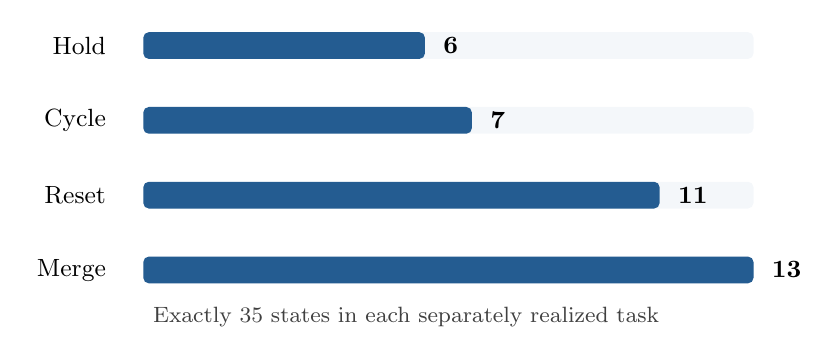
\begin{tikzpicture}[x=1cm,y=1cm,font=\small]
\foreach \lab/\val/\yy in {Hold/6/3.6,Cycle/7/2.65,Reset/11/1.7,Merge/13/.75}{
 \node[anchor=east,font=\small] at (2.0,\yy) {\lab};
 \draw[fill=papergray,draw=none,rounded corners=2pt] (2.35,\yy-.17) rectangle (10.1,\yy+.17);
 \pgfmathsetmacro{\w}{\val/13*7.75}
 \draw[fill=azure,draw=none,rounded corners=2pt] (2.35,\yy-.17) rectangle ({2.35+\w},\yy+.17);
 \node[anchor=west,font=\small\bfseries] at ({2.46+\w},\yy) {\val};
}
\node[anchor=west,font=\footnotesize,text=black!75] at (2.35,.15) {Exactly 35 states in each separately realized task};
\end{tikzpicture}
}
\caption{Four distinct machines with 35 logical states. Exact minimum element counts, respectively, follow from binary storage, Theorem~\ref{thm:capacity}, Theorem~\ref{thm:reset}, and Theorem~\ref{thm:broom}. These are four different designs, not modes of the same machine.}
\label{fig:tasks}
\end{figure}

An interaction-free endpoint also admits a complete statement.
\begin{theorem}[Independent-element memory law]\label{thm:independent}
A finite unary map can be realized without interactions if and only if $f^2=f$. Let $p$ be the number of its fixed points and let $D$ be the size of its largest preimage fiber, including the fixed point. Then
\begin{equation}\label{eq:independent}
\boxed{\Nmin^{(0)}(f)=D-1+\ceil{\log_2p}.}
\end{equation}
The one-state identity uses zero switches by convention.
\end{theorem}
\begin{proof}
An independent bit, driven by the same pulse from the same baseline, either retains its value or becomes permanently on; no other designated net operation can occur under the one-flip budget. Thus the full map is idempotent. Let $r$ denote the number of latch bits that can be added. Each preimage of a fixed state can omit at most one such bit, so $D\le r+1$. All $p$ different fixed codes contain those $r$ bits and require at least $\ceil{\log_2p}$ remaining label bits. For equality choose $D-1$ latch bits and that number of label bits. Each leaf omits a distinct latch bit, while its destination contains them all. Identical independent thresholds restore the missing bit on the pulse and never disturb the labels.
\end{proof}

Figure~\ref{fig:tasks} summarizes the main lesson. The task's \emph{transition structure}, not merely its number of logical states, changes the exact minimum memory cost. For $m=35$, hold, cycle, reset and two-stage merge require respectively 6, 7, 11 and 13 switches.

\section{An exact switch--interaction frontier for reset}\label{sec:frontier}
A result such as Theorem~\ref{thm:reset} minimizes switches without asking what interactions are needed. To expose that hidden cost, fix a switch budget $n$ and interaction degree $d$ and minimize the directed support $K$ from \eqref{eq:costs}.

Let $T$ be a reset target with $k$ on bits and $e=n-k$ off bits. Put $M=m-1$. At most $k$ sources can be immediate subsets of $T$ without using interactions. The remaining
\begin{equation}\label{eq:qdef}
 q=\max(0,M-k)
\end{equation}
require exchanges $T-j+r$, with $j\in T$ and $r\notin T$. The capacity condition is $M\le k(e+1)$.

For one erroneous outside bit $r$, the downward threshold must change sign when the missing target bit $j$ is restored:
\begin{equation}\label{eq:thresholdjump}
 U_r^-(T\setminus\{j\})<0<U_r^-(T).
\end{equation}
Each required $j$ must occur in at least one active monomial of recipient $r$; a degree-$d$ term can cover at most $d$ such indices. This converts the physical switch problem into a finite incidence-cover problem.

Write $k=ad+b$ with integers $a\ge0$ and $0\le b<d$. With $e$ outside-bit rows and a budget of $C$ interaction terms, the maximum coverable number of required $(r,j)$ incidences is
\begin{equation}\label{eq:F}
 F_{k,e,d}(C)=d\min(C,ea)+b\min\{e,\max(0,C-ea)\}.
\end{equation}
Define $\kappa(q;k,e,d)$ as the least $C$ for which $F_{k,e,d}(C)\ge q$, with $\kappa(0;k,e,d)=0$ and $\kappa=\infty$ for $q>ke$.

\begin{theorem}[Exact reset resource frontier]\label{thm:frontier}
For $m\ge2$, $n\ge1$ and $d\ge1$, the exact minimum number of directed nonconstant threshold monomials realizing $R_m$ with at most $n$ switches and degree at most $d$ is
\begin{equation}\label{eq:frontier}
\boxed{\Kmin(R_m;n,d)=\min_{\substack{1\le k\le n\\M\le k(n-k+1)}}\kappa(\max(0,M-k);k,n-k,d),}\quad M=m-1.
\end{equation}
An empty minimum is infeasible. The optimum admits nonnegative common shifts, a uniform hysteresis span, separated bands and an avalanche-free realization. At degree zero, reset is feasible precisely when $n\ge m-1$, with $K=0$.
\end{theorem}
\begin{proof}
The incoming-code count enforces $M\le k(e+1)$, and the sign changes in \eqref{eq:thresholdjump} require $q$ distinct source incidences among the $e$ outside recipients. A row can cover at most $d$ indices per monomial. Greedily using $a$ full $d$-subsets in each row before any remainder gives the maximal possible cover function \eqref{eq:F}, hence the stated lower bound.

For attainment, include $T$, the required immediate subsets, and distribute exactly $q$ exchange sources across outside recipients according to the optimal cover. Partition the selected target indices for each recipient $r$ into groups $G$ of size at most $d$, with $g_r$ groups. Choose $0<\eta_i<1/8$, $W=2\max_r g_r+4$ (with $\max\emptyset=0$), and pulse $0\nearrow3\searrow0$. Use $U_j^+=2+\eta_j$, $U_j^-=U_j^+-W$ for $j\in T$ and
\begin{equation}\label{eq:frontconstruct}
 U_r^-=1-2g_r+\eta_r+2\sum_G\prod_{j\in G}s_j,\qquad U_r^+=U_r^-+W \quad(r\notin T).
\end{equation}
The represented erroneous bit has at least one inactive group before restoration, so it stays on at the baseline. After the missing target bit switches on, all groups are active and its downward threshold is positive, removing the erroneous bit on descent. Off outside bits have upward thresholds above the peak; all bands are separated. The construction has exactly $\sum_rg_r=\kappa$ active monomial positions. The zero-degree endpoint follows from Theorem~\ref{thm:independent}.
\end{proof}

\begin{figure}[ht]
\centering\resizebox{\linewidth}{!}{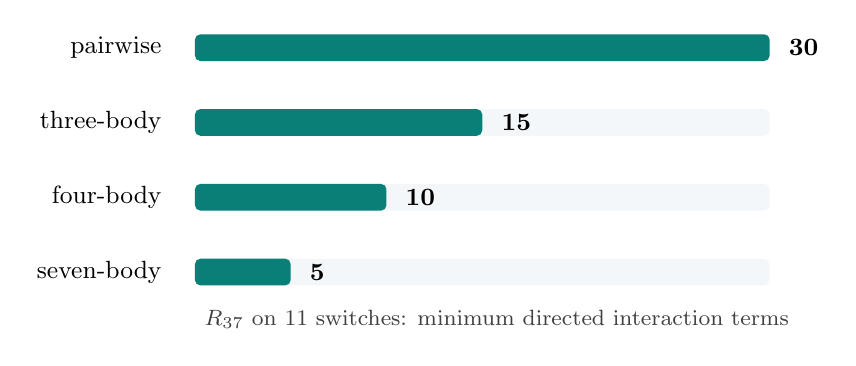
\begin{tikzpicture}[x=1cm,y=1cm,font=\small]
\foreach \arity/\K/\yy in {pairwise/30/3.6,three-body/15/2.65,four-body/10/1.7,seven-body/5/.75}{
 \node[anchor=east,font=\small] at (2.65,\yy) {\arity};
 \draw[fill=papergray,draw=none,rounded corners=2pt] (2.95,\yy-.17) rectangle (10.25,\yy+.17);
 \pgfmathsetmacro{\w}{\K/30*7.30}
 \draw[fill=jade,draw=none,rounded corners=2pt] (2.95,\yy-.17) rectangle ({2.95+\w},\yy+.17);
 \node[anchor=west,font=\small\bfseries] at ({3.07+\w},\yy) {\K};
}
\node[anchor=west,font=\footnotesize,text=black!75] at (2.95,.15) {$R_{37}$ on 11 switches: minimum directed interaction terms};
\end{tikzpicture}
}
\caption{An exact slice of the resource frontier: a 37-state one-pulse reset on 11 hysterons. Higher interaction order reduces the minimum number of directed terms, but not necessarily the total physical coupling effort.}
\label{fig:frontier}
\end{figure}

For $R_{37}$, eleven switches are minimal. They require $k=6$, $e=5$, and $q=30$ at this budget. Theorem~\ref{thm:frontier} gives precisely $K=30,15,10,5$ for maximum body orders $2,3,4,7$, respectively. With no interactions, 36 switches are needed.

A second cost captures what the term count conceals.
\begin{corollary}[Exact reset incidence bound]\label{cor:incidence}
For a feasible switch budget, let $k_{\max}$ be the largest integer $k\in[1,n]$ satisfying $m-1\le k(n-k+1)$. For every available interaction degree $d\ge1$, the minimum weighted source-incidence count is
\begin{equation}\label{eq:incidence}
\boxed{I_{\min}(R_m;n)=\max(0,m-1-k_{\max}).}
\end{equation}
\end{corollary}
\begin{proof}
Every required $(r,j)$ in \eqref{eq:thresholdjump} must occur in the support of a monomial; counting source appearances gives $I\ge q$. Taking the largest feasible $k$ minimizes $q$. The pairwise version of \eqref{eq:frontconstruct} uses exactly one appearance per required pair, attaining equality.
\end{proof}

For the 37-state, eleven-switch example all four optimal term-support designs have $I=30$. Higher-order interactions combine several dependencies into one monomial. They do not erase those dependencies. In particular, an interaction term is a formal coefficient, not a unit of wire length, gate area, or energy.

\section{Interaction order can save memory}\label{sec:separation}
The frontier shows a precise support tradeoff for reset. A different phenomenon occurs when the \emph{number of switches itself} drops upon allowing a higher interaction degree.

Consider the following seven-state map:
\begin{equation}\label{eq:seven}
 C\mapsto A\mapsto R,\qquad B\mapsto R,\qquad R,X,Y,Z\text{ fixed}.
\end{equation}
\begin{figure}[ht]
\centering\resizebox{\linewidth}{!}{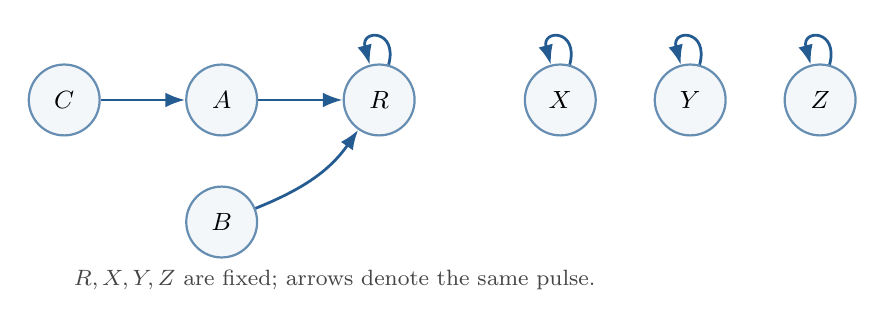
\begin{tikzpicture}[>=Latex,x=1cm,y=1cm,font=\small]
\tikzset{state/.style={circle,draw=azure!70,fill=azure!5,thick,minimum size=9mm,inner sep=0pt,font=\small\bfseries}, edge/.style={-{Latex[length=2.5mm]},draw=azure,line width=1pt}}
\node[state] (C) at (0,1.0) {$C$};
\node[state] (A) at (2.0,1.0) {$A$};
\node[state] (R) at (4.0,1.0) {$R$};
\node[state] (B) at (2.0,-.55) {$B$};
\draw[edge] (C)--(A);\draw[edge] (A)--(R);\draw[edge] (B) to[out=22,in=235] (R);
\node[state] (X) at (6.3,1.0) {$X$};
\node[state] (Y) at (7.95,1.0) {$Y$};
\node[state] (Z) at (9.6,1.0) {$Z$};
\foreach \u in {R,X,Y,Z} {\draw[edge] (\u) to[out=75,in=105,looseness=5] (\u);}
\node[font=\footnotesize,text=black!73,anchor=west] at (0,-1.28) {$R,X,Y,Z$ are fixed; arrows denote the same pulse.};
\end{tikzpicture}
}
\caption{The seven-state task in \eqref{eq:seven}. All arrows represent the same repeated pulse; the four looped states are fixed points.}
\label{fig:seven}
\end{figure}

\begin{theorem}[Seven-state interaction-order separation]\label{thm:seven}
For the map \eqref{eq:seven}, exactly four switches are necessary and sufficient with affine pairwise thresholds, while exactly three are necessary and sufficient with quadratic three-body thresholds. At three switches, the minimum directed monomial-support cost is $K=7$. The seven-state task is the smallest logical-state size exhibiting an affine-versus-quadratic switch-count gap in the complete finite classification performed here.
\end{theorem}
\begin{proof}
Two switches cannot encode seven different states. Suppose there are three. The edge $C\to A$ has a nonfixed target and must be an exchange. Its peak is not a logical code; since seven of the eight cube vertices are codes, this is the unique nonlogical vertex. Neither $A\to R$ nor $B\to R$ can be an exchange: either would use this same nonlogical peak but require descent to $R$ instead of $A$. Both are therefore additions. Write $k=|C(A)|=|C(B)|=|C(C)|$, so $|C(R)|=k+1$. The existence of three distinct weight-$k$ codes forces $k=1$ or $2$. If $k=2$, the exchange peak of $C\to A$ is the full three-set, which is also $C(R)$, a contradiction. Hence $k=1$. Relabeling the bits gives
\[
 C(R)=\{a,b\},\qquad C(A)=\{a\},\qquad C(B)=\{b\},\qquad C(C)=\{c\}.
\]
The unique nonlogical peak is $\{a,c\}$; injection forces the remaining fixed codes to be $\emptyset$, $\{b,c\}$ and $\{a,b,c\}$.

These fixed codes cannot exploit returning excursions. Any addition from $\emptyset$ reaches one of the three baseline-stable singleton codes, and an addition from $\{b,c\}$ reaches the baseline-stable full code. Such a peak has no downward threshold above $L$, so it cannot return to its starting code. The full code has no off bit. Thus all three are physically silent on the operating pulse.

Let $t(b,c)=U_a^+(b,c)$. The transitions from $B$ and $C$ must add $a$, while the fixed codes $\emptyset$ and $\{b,c\}$ must keep it off. Consequently
\begin{equation}\label{eq:xor}
 t(0,0)>H,\qquad t(1,0)<H,\qquad t(0,1)<H,\qquad t(1,1)>H.
\end{equation}
Every affine function satisfies $t(0,0)+t(1,1)=t(1,0)+t(0,1)$, contradicting these strict inequalities. This rules out three-switch affine realizations even with signed coefficients, independent threshold branches and potentially returning fixed-state excursions.

The quadratic upper bound uses $L=0,H=3$, offsets $\eta_a=1/32$, $\eta_b=2/32$, $\eta_c=3/32$, and
\begin{align}\label{eq:sevenparams}
 U_a^+&=4-2b-2c+4bc+\eta_a,\\
 U_b^+&=4-2a+2c+\eta_b,\\
 U_c^+&=4+7a-7ab+\eta_c,\qquad U_i^-=U_i^+-10.\nonumber
\end{align}
The codes are $C(R)=\{a,b\}$, $C(A)=\{a\}$, $C(B)=\{b\}$, $C(C)=\{c\}$, $C(X)=\emptyset$, $C(Y)=\{b,c\}$, $C(Z)=\{a,b,c\}$. Exact substitution proves every pulse and a positive span in every environment. A four-switch affine construction is listed in Appendix~\ref{app:designs}, completing the count minima.

For the support lower bound, the four inequalities for $U_a^+$ force nonzero coefficients at all three positions $b$, $c$ and $bc$. In the $b$ row, $U_b^+(0,0)>H>U_b^+(1,0)$ forces a nonzero $a$ term. At the peak $\{a,c\}$, a second addition is forbidden, so $U_b^+(1,1)>H$; comparison with $U_b^+(1,0)<H$ forces at least one further position, $c$ or $ac$. In the $c$ row, baseline stability of $\{c\}$ and the deletion from $\{a,c\}$ give $U_c^-(0,0)<L<U_c^-(1,0)$, forcing a nonzero $a$ term. Stability of the fixed full code gives $U_c^-(1,1)<L$, forcing at least one additional position, $b$ or $ab$. The resource measure counts the union of positions on the two branches, so these arguments prove $K\ge3+2+2=7$ even for independent branch coefficients. Formula~\eqref{eq:sevenparams} attains seven. The smallest-logical-state-size assertion additionally relies on the complete finite classification described in Section~\ref{sec:algorithm}.
\end{proof}

The signed quadratic construction is not monotone in every other bit. Its global span is ten, but the demonstrated operating robustness does not imply avalanche-freedom under arbitrary off-protocol driving. The distinction is relevant for mechanical embedding.

\begin{theorem}[Decimal counter order separation]\label{thm:decimal}
For a ten-state periodic counter,
\begin{equation}\label{eq:decimal}
\boxed{\Nmin^{(1)}(10)=6,\qquad \Nmin^{(2)}(10)=5.}
\end{equation}
The six-switch affine design and the five-switch quadratic design may each use uniform widths and nonnegative common interaction shifts.
\end{theorem}
\begin{proof}
The capacity inequality rules out four or fewer switches for a ten-cycle. A five-switch counter must use all ten weight-two baseline states and all ten weight-three peaks. The two halves of its pulse therefore induce perfect incidence matchings between the two Boolean layers. Order each layer by increasing binary mask. Among the sixty perfect incidence matchings in these fixed orders, fifty-four are odd and six are even. Every even matching has the same summed affine feature vector: each recipient appears twice and each ordered recipient/source pair once. Hence every even matching has the same total affine switching score. A strictly winning affine selector cannot be even, since another distinct even matching has the same summed score. The inverse of the downward matching is represented in the same two layer orders and uses the same recipient/environment incidence features. A strict downward winner cannot give an even matching either: summing its strict maximizing inequalities over the matched peaks would contradict the identical total feature vector of another even matching. The full pulse is the composition of two odd matchings, hence an even permutation. But a single ten-cycle is odd. This proves the pairwise impossibility. The two explicit parameter systems and complete winning inequalities are provided in Appendix~\ref{app:designs} and the accompanying certificates.
\end{proof}

The five-switch affine counter has a sharp maximum period of nine: a period-nine witness is supplied, and Theorems~\ref{thm:decimal} and \ref{thm:capacity} excludes all longer periods.

These results do not say that three-body interactions are universally superior. They show that \emph{under the stated switching budget}, increasing allowable interaction order can lower the minimum element count for particular transition maps. The seven-state separation is the smaller forced-encoding example; the ten-cycle is a periodic separation with monotone positive-coefficient upper witnesses.

\section{Algorithms, certificates, and other restrictions}\label{sec:algorithm}
The theorems above give exact formulas for particular task families. For an arbitrary finite unary map, a general closed formula for minimum switch count or the complete resource profile remains unavailable. There is nevertheless a complete \emph{finite} decision procedure for any fixed budgets.

\begin{theorem}[Budgeted finite synthesis]\label{thm:synthesis}
Given a finite unary map, an element budget $n$, a maximum monomial degree $d$, and permitted directed monomial positions (or a finite support budget), realizability reduces to a finite family of rational linear-feasibility systems. One may additionally impose common branch shifts, uniform hysteresis spans and coefficient sign restrictions. Exhaustive exact resolution of these systems decides the prescribed finite resource problem.
\end{theorem}
\begin{proof}
Enumerate injective state encodings. Reject encodings that violate Theorem~\ref{thm:criterion}. Enumerate the possible up/down return excursion at each logical fixed state; such excursions cannot be assumed absent when proving degree-restricted minima. For the requested support set, write the threshold values using \eqref{eq:poly}. Every condition for initial stability, the first upward winner, the absence of further upward events, the downward winner, post-flip stability and the final endpoint is linear in the coefficients and pulse height. So are the all-environment span conditions, sign restrictions and equalities imposing common shifts. Normalize $L=0$ and scale any strictly feasible system to make the strict margins at least one. Each finite case becomes a rational system $Ax\ge b$, decidable by exact linear elimination. Feasible rational vectors give parameter witnesses; infeasible systems admit certificates of the alternative \citep{farkas1902}. Enumeration is finite, though not necessarily computationally practical.
\end{proof}

For small tasks, the companion implementation enumerates code geometry, solves candidate linear systems and verifies rational witnesses. An infeasibility certificate has nonnegative weights $y$ such that $A^\top y=0$ and $b^\top y>0$ for the proposed $Ax\ge b$. A search timeout or failed numerical reconstruction is explicitly an \emph{unresolved case}, not evidence of impossibility.

A useful necessary inequality can be obtained before any linear solve. Join logical states $x$ and $f(x)$ when $f(x)$ is nonfixed. Each resulting cohort must occupy a common Boolean-weight layer. If cohort $B$ is permitted only weights $W_B$, then for any collection $\mathcal B$ of cohorts,
\begin{equation}\label{eq:cohort}
 \sum_{B\in\mathcal B}|B|\le\sum_{k\in\cup_{B\in\mathcal B}W_B}\binom nk.
\end{equation}
This layer-packing obstruction rules out some codes which pass separate storage and fan-in bounds. It is necessary, not claimed sufficient.

\begin{theorem}[Sparse one-hot pairwise realization]\label{thm:sparse}
For every unary map $f$ without a two-cycle, let $e_f$ count its nonfixed directed edges. There is a common-shift, uniform-span pairwise realization using $|X|$ switches and at most $3e_f$ nonconstant directed terms, with coefficients drawn from $\{-2,2,4\}$.
\end{theorem}
\begin{proof}
Use the one-hot codes $C(i)=\{i\}$, initially setting every off-diagonal entry of $J$ to zero. For every nonfixed edge $i\to j$, set $J_{ji}=-2$ and $J_{ij}=4$. These assignments conflict only for a directed two-cycle. For every three-distinct-state chain $i\to j\to r$, replace $J_{ri}$ by $\max\{2,J_{ri}\}$. This entry cannot be negative: a negative entry would require $f(i)=r$, whereas $f(i)=j$. Thus all nonzero entries belong to $\{-2,2,4\}$.

Put
\[
 P=\max_i\sum_{j\ne i}\max(J_{ij},0),\qquad
 N=\min_i\sum_{j\ne i}\min(J_{ij},0),\qquad
 B=\max\{4,1+P-N\}.
\]
Choose distinct $0<\eta_i<1/8$, and set
\[
 U_i^+=B+\eta_i+\sum_{j\ne i}J_{ij}s_j,\qquad
 U_i^-=-3+\eta_i+\sum_{j\ne i}J_{ij}s_j,
 \qquad L=0,\quad H=B-1.
\]
The common span is $B+3$. In every Boolean environment,
$U_i^+\ge B+N+\eta_i$ and $U_i^-\le-3+P+\eta_i$, so all upward thresholds exceed all downward thresholds.

At $\{i\}$, its unique successor $j=f(i)\ne i$ has upward threshold $B-2+\eta_j<H$, while every other off bit has threshold at least $B+\eta_r>H$. If $i$ is fixed there is no negative entry in column $i$, and no addition occurs. At a used peak $\{i,j\}$, an off bit $r$ can have a negative contribution only when $j\to r$; the skipping correction then guarantees $J_{ri}+J_{rj}\ge0$. Hence no second addition occurs. The old bit $i$ has downward threshold $1+\eta_i$, whereas the newly added bit $j$ has threshold $-5+\eta_j$. Thus descent removes exactly $i$. After this deletion, the remaining on bit has threshold $-3+\eta_j<0$, and every off bit has upward threshold at least $B-2+\eta_r>1+\eta_i$, so the final state remains stable to the baseline.

There are at most two assigned directed positions per nonfixed edge and one additional position per eligible two-step chain. Since each such chain starts at a nonfixed edge, $K\le3e_f$.
\end{proof}

This intentionally trades memory for sparse coupling support. It is not a claim that $|X|$ switches or $3e_f$ terms are jointly optimal. Nor does it guarantee arbitrary off-orbit avalanche-freedom for signed threshold shifts.

\subsection{Two limitations of the input protocol}
The switching budget also restricts control and reciprocity.

\begin{proposition}[Amplitude-only inputs]\label{prop:amplitude}
Allow several input symbols distinguished solely by their positive peak amplitudes $H_1<\cdots<H_r$ and sharing the same baseline. If each admitted pulse obeys the budget, then from any given logical state, smaller amplitudes may hold that state, but every amplitude that changes it must produce the \emph{same} nonself successor. A finite amplitude-input table is realizable precisely when each row has such a hold-prefix/advance-suffix structure and the highest-amplitude successor map has no directed two-cycle.
\end{proposition}
\begin{proof}
The first upward event from a given state does not depend on how high the pulse will eventually rise. Before it, the state is unchanged; after it, the one-addition budget forbids further upward events. Descending from that unique peak has a unique result. For sufficiency, let $f$ be the highest-amplitude successor map and use one-hot codes. For every nonfixed row $i$, let $g_i$ be its first advancing symbol, put $H_0=L$, and choose $h_i\in(H_{g_i-1},H_{g_i})$. Choose constants $\ell<L<\delta<\min_i h_i$ and $M>H_r$; when there are no nonfixed rows, choose any $L<\delta<H_1$. Start with $U_a^+(E)=M$ and $U_a^-(E)=\ell$ in every environment. For each nonfixed edge $i\to j$, replace
\[
 U_j^+(\{i\})=h_i,\qquad U_i^-(\{j\})=\delta.
\]
The absence of two-cycles makes every used two-bit peak have exactly one designated deletion. At $\{i\}$, symbol $a$ activates $j$ precisely when $a\ge g_i$; no second addition is eligible at $\{i,j\}$, and its unique deletion returns $\{j\}$. After deletion all remaining upward thresholds exceed $\delta$, and the occupied bit has downward threshold $\ell<L$. Every span is positive because all upward thresholds exceed $\delta$ and every downward threshold is at most $\delta$. This realizes the entire table for the prescribed amplitudes.
\end{proof}

A further obstruction holds if one threshold branch is a discrete gradient on the Boolean cube. For example, if the down thresholds satisfy $U_i^-(S)=E(S)-E(S\setminus\{i\})$, the selected deletion in a counter step implies $E(A_{t+1})<E(A_t)$. Energy cannot strictly decrease around a closed cycle. The analogous argument compares successive peaks for an up-gradient branch. Therefore a symmetric affine coupling matrix on either threshold branch forbids these cyclic counters. This concerns the \emph{effective threshold representation} and is not a blanket statement about every passive system with an energy function.

\subsection{Computational cross-checks}
The exact finite classification through seven logical states covers 550 transition-map isomorphism types, corresponding to 873,612 labeled maps: 224 types contain a forbidden two-cycle, while 326 types are realizable. The computed unrestricted and affine minima agree through six states; at seven states the only separated type is the map \eqref{eq:seven}. The complete lower-dimensional encoding enumeration for that map examines 40,320 injections into the three-cube and yields 36 geometry-consistent encodings, all equivalent under the stated relabelings. Exact linear certificates cover its affine infeasibility.

The audit of the prior event checker found a specific implementation defect. Checking only the designated pulse traces could accept a model with a nonpositive hysteresis span in an environment not visited by those traces. The repaired validation path checks \eqref{eq:span} globally when feasible, or proves it symbolically for common-shift models. Earlier explicit designs pass the stronger checks. This correction matters because \emph{orbit verification is not model validation}; tests of a claimed physical model must do both.

The reproducibility archive includes all three stages of construction scripts and finite certificates, a standardized verification entry point, exact event traces, deliberate negative tests and raw research logs. Numerical search is used for discovery only; exact witnesses and algebraic lower bounds carry the stated conclusions. Computation checks examples and enumeration, while the all-size statements rest on their written proofs.

\section{Discussion and scope}\label{sec:discussion}
There are three complementary outcomes.
\begin{enumerate}
\item \textbf{Existence is simpler than optimization.} A two-cycle is the only unary obstruction with unrestricted size, and pairwise couplings suffice for every other unary map. But the minimum switch count can depend sharply on the task's transition structure.
\item \textbf{Memory cost is not state count.} Cycle capacity follows adjacent-layer geometry; one-pulse reset cost follows in-degree geometry; two-stage merging pays an additional reserved-peak cost. These lower bounds hold regardless of how complicated the threshold interaction functions are.
\item \textbf{Interaction complexity changes the attainable resource point.} Higher-order terms permit smaller networks for specific tasks and compress the term support for reset, while weighted incidence exposes a dependence that cannot be removed by merely grouping terms together.
\end{enumerate}

These resource coordinates should not be confused with a physical bill of materials. Geometry and sign constraints can make an abstract threshold tensor unrealizable in a chosen spring or rotor mechanism. Concrete mechanical mappings have been developed \citep{shohat2025,paulsen2026}, and controllable three-body effects have been demonstrated \citep{ali2026}, but their available parameter classes are not identical to arbitrary polynomial thresholds. Experimental robustness, thermal fluctuations, coefficient precision, work per pulse and actuation speed remain outside the present theorems. Large-span switching dynamics have also been studied independently \citep{teunisse2026span}.

The mathematical results advanced here are model-specific exact minima, constructions, resource frontiers and restricted-interaction separations. General hysteron transition-graph synthesis \citep{teunisse2025}, finite-state encoding \citep{ahmad2000}, and Boolean-lattice cycle existence \citep{mutzesu2017,mutze2016} are established ingredients. Duffus, Sands and Woodrow \citep{duffus1988} give a separate obstruction for cycles formed from lexicographic matchings. Our additional restrictions concern individual flip counts and exact resource minima.

The general optimum $\Nmin^{(d)}(f)$ for large arbitrary transition graphs, the full switch--degree--support frontier, efficient solution complexity, multi-field control, and faithful physical realization are open beyond the classes solved here. Even an exact finite decision method need not scale favorably. Those are natural next problems, but they are not needed to state the present restricted theory accurately.

\section{Conclusion}
A memory device's information capacity specifies how many states it can represent. Under a tightly limited physical input protocol, the transitions it must perform impose additional, mathematically quantifiable constraints. We have shown that geometry yields universal obstructions; those obstructions lead to sharp switch minima for cycles, resets and merging tasks; and interaction order and support determine further, independently measurable costs. The resulting resource profile unifies exact construction, impossibility and optimization within one model. Its purpose is not to replace established finite-state or hysteron theory, but to make the material cost of a prescribed transition structure an explicit, checkable mathematical question.

\section*{Data and reproducibility}
The accompanying source archive contains the LaTeX manuscript, figure sources, constructive parameters, proof certificates, exact event simulator, model validator, regression tests and reproduction instructions. Code and certificate checks require Python 3.10 or later and only the standard library. The initial discovery scripts may require numerical optimization packages; they are not prerequisites for checking the supplied exact results. The code, machine-readable witnesses and exact certificates are supplied in the accompanying review archive. The reviewer guide records the scope and provenance of the checks.

\appendix
\section{The cycle compiler, explicitly}\label{app:compiler}
Let $A_t,P_t,A_{t+1}$ be successive low--peak--low configurations of an alternating cycle between layers $k,k+1$, with $P_t=A_t\cup\{p_t\}=A_{t+1}\cup\{r_t\}$. For every $k$-set $A$ excluding recipient $i$, assign
\begin{equation}\label{eq:labels}
 c_{i,A}=\begin{cases}0,& A\to A+i\ \text{is a cycle addition},\\4,& A+i\to A\ \text{is a cycle deletion},\\2,&\text{otherwise}.\end{cases}
\end{equation}
Put $f_i(s)=\sum_{|A|=k}c_{i,A}\prod_{j\in A}s_j$. Set $B=2\binom{n-1}{k}$ for any closed alternating cycle, $U_i^+=B+\eta_i+f_i$ and $U_i^-=-2+\eta_i+f_i$, with distinct $0<\eta_i<1/4$, and drive $0\nearrow B+1\searrow0$. Each row has one zero and one four for every balanced recipient addition/deletion, so its coefficient sum remains $B$; hence $0\le f_i\le B$.

At a lower state $A_t$, off candidate $i$ sees exactly $c_{i,A_t}$. The chosen addition has threshold $B+\eta_{p_t}$ and every competitor at least $B+2$. At the peak $P_t$, off candidates remain above the driven maximum, while on candidates see one coefficient from the subset obtained by removing themselves. The unique selected deletion has threshold $2+\eta_{r_t}$; competitors have threshold at most $\eta_i$. After the deletion every remaining on threshold is negative. The global upward/downward bands are disjoint and monotonicity forbids an avalanche. This proves Theorem~\ref{thm:capacity} upon invoking \citep[Thm.~9]{mutzesu2017}.

A saturated alternative uses $f_i(E)=\max(\{c_{i,A}:A\subseteq E,|A|=k\}\cup\{0\})$ and thresholds $U_i^+=4+\eta_i+f_i$, $U_i^-=-2+\eta_i+f_i$, driven by the fixed pulse $0\nearrow5\searrow0$ with width six. It bounds all effective shifts between zero and four, but its expanded multilinear polynomial may have higher degree than $k$.

\section{Construction details for merging}\label{app:reset}
Choose intermediate $T$ of weight $k$, reserved outside bit $p$, and $e=n-k-1$ other outside bits $E$. Include leaf codes $T-j+r$ for pairs $(j,r)\in T\times E$ and fixed root $T+p$. Take $W=\max(2k+4,2e+4)$, $L=0$, $H=3$, and distinct $0<\eta_i<1/8$. For $j\in T$, set $U_j^+=2+\eta_j$ and $U_j^-=U_j^+-W$. For $r\in E$, set
\[
 U_r^-=1-2k+\eta_r+2\sum_{j\in T}s_j,\quad U_r^+=U_r^-+W.
\]
For the reserved bit put $U_p^+=2+\eta_p+2\sum_{r\in E}s_r$ and $U_p^-=U_p^+-W$. A leaf contains one unwanted $r$ and lacks one $j$; the pulse adds $j$ and then removes $r$. From $T$, the next pulse adds $p$ and stops. Every other candidate lies above the peak threshold. All coefficients that are present are nonnegative and the branch spans are equal.

\section{Finite construction data for the interaction-order separations}\label{app:designs}
For the ten-state quadratic counter, $n=5$, $L=0$, $H=13$, $\eta_i=i/100$, and $U_i^+=12+\eta_i+f_i$, $U_i^-=-2+\eta_i+f_i$, with
\begin{align*}
 f_1&=4s_2s_3+4s_2s_4+2s_3s_5+2s_4s_5,\\
 f_2&=2s_1s_3+2s_1s_5+4s_3s_4+4s_4s_5,\\
 f_3&=2s_1s_4+4s_1s_5+2s_2s_4+4s_2s_5,\\
 f_4&=2s_1s_2+4s_1s_3+2s_2s_5+4s_3s_5,\\
 f_5&=4s_1s_2+4s_1s_4+2s_2s_3+2s_3s_4.
\end{align*}
Its baseline cycle is
\[
\begin{aligned}
 \{1,2\}&\to\{2,3\}\to\{3,4\}\to\{1,3\}\to\{1,5\}\to\{1,4\}\\
 &\to\{2,4\}\to\{4,5\}\to\{3,5\}\to\{2,5\}\to\{1,2\}.
\end{aligned}
\]
The companion exact checker verifies the unique up and down events at all ten steps and every environment-dependent positive span.

For the six-switch affine decimal counter use $U_i^+=a_i+i/100+\sum_{j\ne i}J_{ij}s_j$ and $U_i^-=b_i+i/100+\sum_{j\ne i}J_{ij}s_j$, with $L=0,H=107$,
\begin{gather*}
 a=(75,79,75,75,86,84),\qquad b=a-104(1,1,1,1,1,1),\\
 J=\begin{pmatrix}
0&14&21&2&13&24\\20&0&5&37&8&20\\10&17&0&24&17&20\\24&15&5&0&17&10\\13&13&5&12&0&1\\8&15&10&10&15&0
\end{pmatrix}.
\end{gather*}
The orbit and exact event traces are provided in the machine-readable data file. Its span is 104; every off-diagonal interaction is positive. For the seven-state affine upper bound, use four bits, $L=0,H=642$,
\[
 a=(323,804,1125,486),\quad U_i^+=a_i+\sum_jJ_{ij}s_j,\quad U_i^-=U_i^+-1282,
\]
\[
 J=\begin{pmatrix}0&160&320&480\\640&0&-320&0\\-320&320&0&-320\\320&160&160&0\end{pmatrix},
\]
in integer-scaled parameter units (scale factor 80); no additional offsets are needed for this witness. The logical state masks in order $(R,A,B,C,X,Y,Z)$ are $(1,2,0,4,5,7,8)$. These explicit parameters give the upper bound, while Theorem~\ref{thm:seven} gives the matching lower bound.

\section{Lifting an alternating cycle}\label{app:lift}
Write a period-$Q$ alternating cycle in the cube as $A_0,P_0,A_1,P_1,\ldots,A_{Q-1},P_{Q-1}$, with distinct low and peak states. Introduce two fresh bits $x$ and $y$. For an even desired period $q=2t$, take the low-state sequence
\[
 A_0+x, A_1+x,\ldots,A_{t-1}+x,A_{t-1}+y,\ldots,A_0+y.
\]
Connect consecutive states by copies of the original peaks in their appropriate slice and by the two rungs $A_{t-1}+x+y$ and $A_0+x+y$. For an odd period $q=2t+1$, replace the closing rung with the additional low state $P_{Q-1}$ containing neither fresh bit and use peaks $P_{Q-1}+y$ and $P_{Q-1}+x$. All low and peak vertices remain distinct for $3\le q\le2Q+1$; the new lower layer has weight $k+1$. Applying Appendix~\ref{app:compiler} completes the construction.

\clearpage
\begingroup
\small
\setlength{\bibsep}{1pt}

\section*{Reproducibility and Disclosure}
\addcontentsline{toc}{section}{Reproducibility and Disclosure}
The source manuscript, native TikZ figures, rational witness certificates, and exact Python verification scripts are archived in the public Open-Research repository (\url{https://github.com/Rtx09x/Open-Research/tree/main/applied-physics/hysteretic-state-machines}, release reference \texttt{7099139817e621ce40074813c163389f3eefe6a3}) and bound by SHA-256 manifests. Running \texttt{repro/original/src/verify.py} and \texttt{repro/original/src/verify\_reset.py} with assertions enabled checks the 16 finite witness and enumeration checks (including the 60-matching enumeration, 16 Hamiltonian dual certificates, 5-switch three-body and 6-switch pairwise decimal counters, and nominal reset protocols). Finite computational checks corroborate the explicit constructions and small-$n$ bounds; the general-$n$ theorems rest on the analytic proofs in Sections~\ref{sec:real}--\ref{sec:frontier}. All results apply strictly to the idealized quasistatic switching-threshold model; no experimental hardware fabrication or physical realization feasibility is claimed. This manuscript was developed with AI-assisted research and drafting workflows.

\bibliographystyle{plainnat}
\bibliography{references}
\endgroup
\end{document}
